\chapter{仮想環境における大規模配管設備での検証実験}
第4章では実環境においてアイソメ図作成を試みたが、小規模な配管設備での実験であったため、本章では仮想環境において大規模な配管設備でアイソメ図作成を行う。

\section{データセット収集}
\subsection{仮想環境構築}
仮想環境の構築には、Unityを使用する。Unityは、3Dモデルの読み込みやカメラの画像取得など、仮想環境の構築に必要な機能が備わっている。
本検証に用いた大規模配管設備を導入し、RGB画像とDepth画像を取得した。
仮想環境における画像の取得にはカメラの内部パラメータを設定できるため、実環境に用いたセンサのパラメータを設定することが可能である。
図\ref{fig:f1}には、例としてAzure Kinect DKの内部パラメータを指定して取得した大規模配管設備のRGB-D画像を示した。
\begin{figure}[htbt]
    \centering
    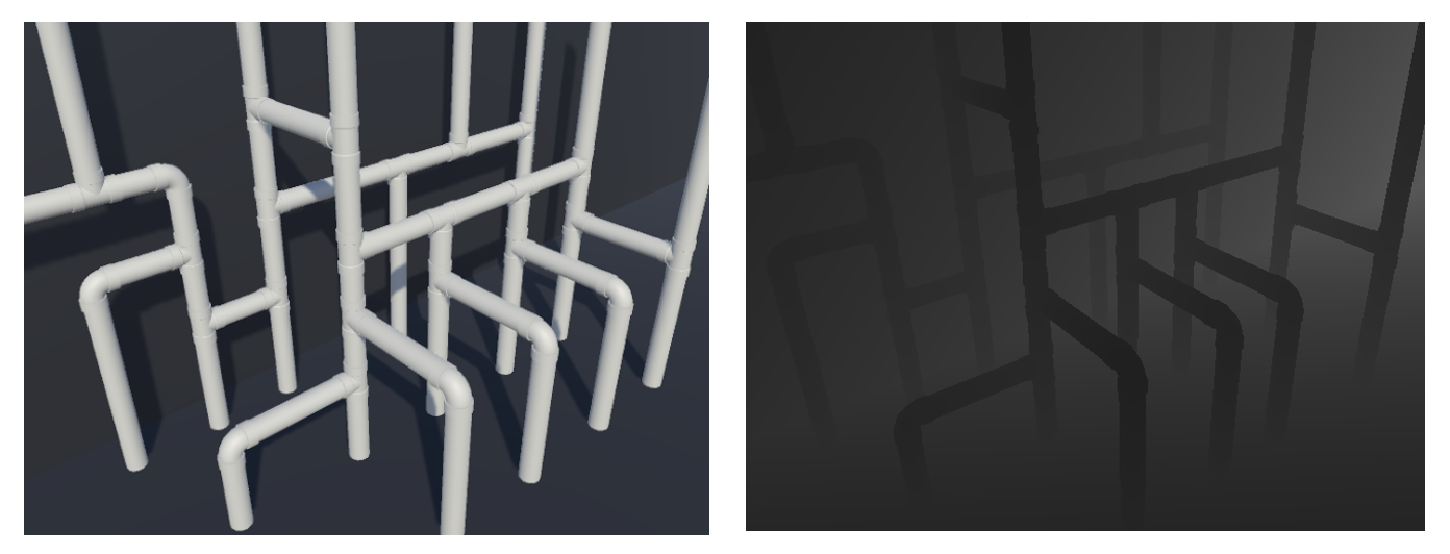
\includegraphics[height=55mm]{Figure/ex_sim.eps}
    \caption{仮想環境で取得した大規模配管設備のRGB-D画像}
    \label{fig:f1}
\end{figure}

\subsection{センサモデルの導入}
仮想環境で取得されるDepth画像には実環境に比べてノイズが存在しない。
そのため、実環境におけるセンサノイズをモデル化し、仮想環境に導入することで、より実環境に近い状況を再現する。
本研究におけるDepthの取得にはノイズ無し(Ideal)とAzure Kinect DK(Sensor A)とRealsense D435i(Sensor B)の3つの条件で行った。
センサモデルの取得には、実環境で0.5mから10.0mの範囲で0.5m間隔で測定した距離と実際の距離との標準偏差を求め、その結果を適切な関数で近似した。
図\ref{fig:f2}には、各センサの標準偏差と測定距離の結果をもとにして近似した結果を示した。
\begin{figure}[htbt]
    \centering
    \includegraphics[height=60mm]{Figure/sensor_model.eps}
    \caption{Sensor Aの線形近似結果(左)とSensor Bの指数近似結果(右)}
    \label{fig:f2}
\end{figure}

Sensor Bの場合、測定距離に対して標準偏差がSensor Aに比べると測定距離が10mの地点では標準偏差に約60倍の差がある。
そのため、Sensor BのセンサモデルはSensor Aに比べてノイズが大きく、Depth画像にばらつきが大きく現れることが予想される。

図\ref{fig:f3}に示したセンサモデルを用いて、Depth画像の取得結果を示した。
画像にはノイズを加えたが、目視ではノイズが確認することができなかったが、6D姿勢推定の結果に影響を与える可能性があるため、アイソメ図生成の精度を検証する。
\begin{figure}[htbt]
    \centering
    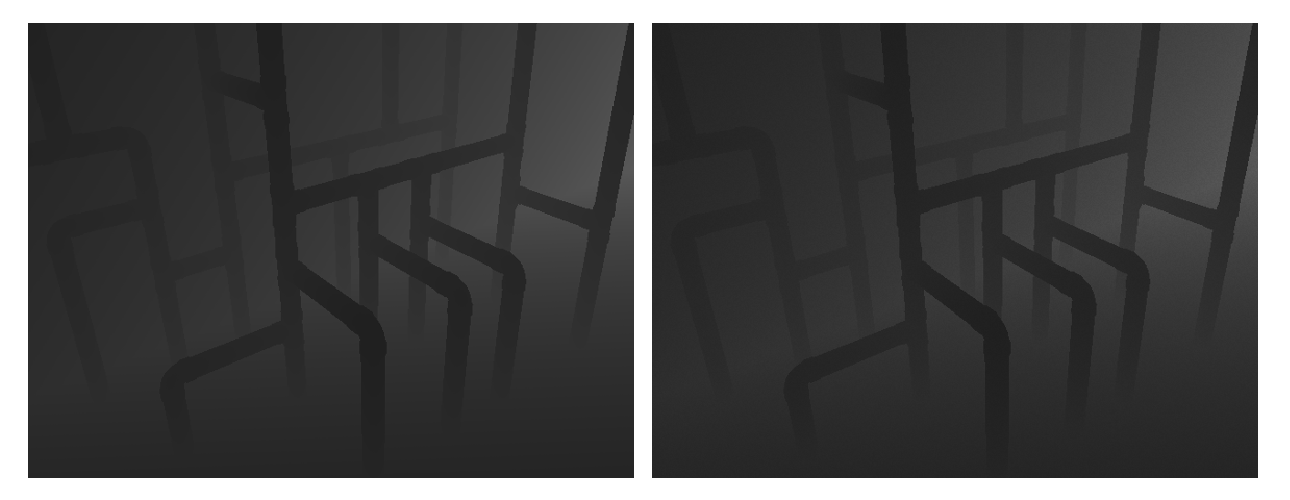
\includegraphics[height=55mm]{Figure/depth_sim.eps}
    \caption{Sensor AモデルによるDepth画像(左)とSensor BモデルによるDepth画像(右)}
    \label{fig:f3}
\end{figure}

\section{評価指標}
評価指標には第4章で述べた6D姿勢推定の評価指標に加え、アイソメ図の評価指標を導入する。
アイソメ図の評価には、Mean Error Distance(MED)とGenerated Line Count(GLC)の2つの指標が用いられる。
アイソメ図の評価におけるMEDは、生成されたアイソメ図の各線分と正解データの線分との平均距離を求めるものである。
この距離は、各線分における誤差を計算し、その平均値を取ることで算出される。

まず、各線分の距離 $d_i$ は、通常、線分の端点間の直線距離を用いて計算される。
例えば、2つの点 $(x_1, y_1)$ と $(x_2, y_2)$ の間のユークリッド距離は、次のように求められる。

\[
d = \sqrt{(x_2 - x_1)^2 + (y_2 - y_1)^2}
\]

この距離を用いて、生成された線分と正解データの対応する線分との誤差を求め、その平均値を取ることで、MEDが算出される。MEDの数式は次のように表される。

\[
MED = \frac{1}{N} \sum_{i=1}^{N} d_i
\]

ここで、$N$は評価対象となる線分の数を示し、$d_i$は第$i$番目の線分における生成されたアイソメ図の線分と正解データの線分との距離である。
MEDの値が小さいほど、正解データとの線分の誤差が少なく、生成されたアイソメ図の精度が高いと評価できる。

一方、GLCは、生成されたアイソメ図と正解データの対応する線分の本数を示す指標である。
この指標は、生成結果が破綻した場合など、MEDだけでは評価が難しい場合に必要となる。
GLCの値が大きいほど、多くの対応線分が正確に生成されているため、アイソメ図の精度が高いと考えられる。

\section{結果と考察}
6D姿勢推定およびアイソメ図生成の結果を図\ref{fig:f4}に示す。
6D姿勢推定では、3Dバウンディングボックスの正解を赤色、推定結果を青色で示しており、これらのボックスが重なるほど推定精度が高いと評価できる。
IdealおよびSensor Aの結果では、推定ボックスが正解ボックスとほぼ一致しており、6D姿勢が高い精度で推定されていることが確認された。
一方、Sensor Bの結果では、多くの配管において推定ボックスが正解ボックスと大きくずれている事例が確認された。
特に、カメラ視点から見えづらい位置にある配管では、姿勢情報の正確な推定が難しく、推定精度が著しく低下していると考えられる。

表5.1に6D姿勢推定の評価結果を示す。
IdealおよびSensor Aでは、TeeおよびElbowの両方で100\%の精度を達成しており、評価指標においても姿勢が正確に推定されていることが分かる。
一方、Sensor BではTeeおよびElbowの両方で精度が低下し、ADD-sucの平均値は42.5\%となった。
この精度低下の要因として、センサモデルにおけるノイズの大きさが挙げられる。
このノイズの影響でDepth画像の取得に問題が生じ、6D姿勢推定におけるポイントマッチングの精度に悪影響を与えたと考えられる。

次に、アイソメ図生成結果について述べる。
生成されたデータと正解データの図面を比較したところ、IdealおよびSensor Aではほぼ一致していることが確認された。
この結果は、6D姿勢推定の精度が高いことから、配管の接続関係を正確に把握できていることを示している。
また、線分のズレが見られないため、距離の誤差が非常に小さいことも確認できた。
一方、Sensor Bでは、生成データと正解データを比較すると、多くの線分にズレが見られ、線分の数が不足していることも確認された。

表5.2にアイソメ図生成の評価結果を示す。
評価結果によると、IdealおよびSensor Aの場合、MEDの値がそれぞれ1.23mm, 1.32mmであった。
これは、正解データと生成データにおいて線分の距離の誤差が非常に小さいことを示しており、アイソメ図生成の精度が高いことが確認できる。
続いて、GLCの値は100\%を示しており、正解データと対応する線分が全て生成できていることを示している。
特に、Sensor Aの場合、このセンサのノイズレベルではアイソメ図を正確に生成可能であることが示唆され、本研究で提案した手法において、このセンサが有効であると考えられる。

一方、Sensor Bの場合、MEDの値は約3.85mであった。
この結果は、IdealやSensor Aと比較して線分の距離誤差が大きいことを示しており、アイソメ図生成の精度が低下していることが確認できる。
さらに、GLCの値が27.7\%であることから、正解データに対応する線分の多くを正確に生成できていないことがわかる。
これにより、このセンサのノイズレベルではアイソメ図生成を正確に行うことが難しいことが明らかになった。
方向ベクトルの表示結果を確認したところ、各配管の3次元空間上の位置には問題がないものの、姿勢が異なる方向を向いているため、接続部のペアリングに誤認識が発生し、誤判定が生じていることがわかった。
また、アイソメ図作成結果における線分の不足の原因として、一部の配管に対してペアが見つからず、それらが地面に設置されているものと誤認識されてしまったことが挙げられる。
その結果、該当する配管の接続探索がスキップされ、生成データに欠損が生じたと考えられる。\\
 以上の結果から、大規模配管設備において、適切なセンサを使用することで、正確なアイソメ図の作成が可能であることが示された。
一方で、センサのノイズレベルが高い場合には、6D姿勢推定結果の精度が低下し、アイソメ図生成結果が破綻してしまう恐れがあることが明らかになった。
したがって、正確なアイソメ図を作成するためには、十分な精度を持つセンサの選定が必要であると考えられる。


\begin{figure}[htbt]
	\centering
	\includegraphics[width=\textwidth]{Figure/result_all_sim.eps}
	\caption{6D姿勢推定とアイソメ図生成結果}
	\label{fig:f4}
\end{figure}

\begin{table}[htbp]
    \centering
    \caption{6D姿勢推定の評価}
    \setlength{\tabcolsep}{5pt}
    \begin{tabular}{|c|c|c|c|c|c|c|c|c|c|}
        \hline
        & \multicolumn{3}{c|}{Ideal} & \multicolumn{3}{c|}{Sensor A} & \multicolumn{3}{c|}{Sensor B} \\ \hline
         & Tee & Elbow & Mean & Tee & Elbow & Mean & Tee & Elbow & Mean \\ \hline
        ADD-suc & 100.0 & 100.0 & 100.0 & 100.0 & 100.0 & 100.0 & 50.0 & 35.0 & 42.5 \\ \hline
        Prj-5-suc & 100.0 & 100.0 & 100.0 & 100.0 & 100.0 & 100.0 & 66.7 & 85.0 & 75.8 \\ \hline
    \end{tabular}
\end{table}



\begin{table}[htbp]
    \centering
    \caption{アイソメ図生成の評価}
    \setlength{\tabcolsep}{5pt} % 列間のスペース設定
    \begin{tabular}{|p{2.0cm}|>{\centering\arraybackslash}p{1.8cm}|>{\centering\arraybackslash}p{1.8cm}|>{\centering\arraybackslash}p{1.8cm}|}
        \hline
        \raggedright & Ideal & Sensor A & Sensor B \\ \hline
        \raggedright MED[mm] & 1.23 & 1.32 & 3.85 \\ \hline
        \raggedright GLC & 100.0 & 100.0 & 27.7 \\ \hline
    \end{tabular}
\end{table}

